\documentclass[12pt, compress, aspectratio=1610]{beamer}

\usetheme{pl}

\usepackage{longtable}
\usepackage{booktabs}
\usepackage{minted}
\usepackage{listings}
\usepackage{color}
\usepackage{fancyvrb}
\newcommand{\VerbBar}{|}
\newcommand{\VERB}{\Verb[commandchars=\\\{\}]}
\DefineVerbatimEnvironment{Highlighting}{Verbatim}{commandchars=\\\{\},fontsize=\small}
% Add ',fontsize=\small' for more characters per line
\usepackage[framemethod=tikz]{mdframed}
\definecolor{shadecolor}{HTML}{EEEEEE}
\mdfsetup{
  backgroundcolor=shadecolor,
  linecolor=shadecolor,
  innerleftmargin=5pt,
  innerrightmargin=5pt,
  leftmargin=-5pt,
  rightmargin=-5pt,
  roundcorner=3pt
}
\newenvironment{Shaded}{\begin{mdframed}}{\end{mdframed}}
\newcommand{\KeywordTok}[1]{\textcolor[rgb]{0.26,0.66,0.93}{\textbf{{#1}}}}
\newcommand{\DataTypeTok}[1]{\textcolor[rgb]{0.74,0.68,0.62}{\underline{{#1}}}}
\newcommand{\DecValTok}[1]{\textcolor[HTML]{558B2F}{{#1}}}
\newcommand{\BaseNTok}[1]{\textcolor[HTML]{558B2F}{{#1}}}
\newcommand{\FloatTok}[1]{\textcolor[HTML]{558B2F}{{#1}}}
\newcommand{\ConstantTok}[1]{\textcolor[rgb]{0.74,0.68,0.62}{{#1}}}
\newcommand{\CharTok}[1]{\textcolor[HTML]{7E57C2}{{#1}}}
\newcommand{\SpecialCharTok}[1]{\textcolor[HTML]{7E57C2}{{#1}}}
\newcommand{\StringTok}[1]{\textcolor[HTML]{7E57C2}{{#1}}}
\newcommand{\VerbatimStringTok}[1]{\textcolor[HTML]{7E57C2}{{#1}}}
\newcommand{\SpecialStringTok}[1]{\textcolor[HTML]{7E57C2}{{#1}}}
\newcommand{\ImportTok}[1]{\textcolor[rgb]{0.74,0.68,0.62}{{#1}}}
\newcommand{\CommentTok}[1]{\textcolor[HTML]{546E7A}{\textit{{#1}}}}
\newcommand{\DocumentationTok}[1]{\textcolor[HTML]{BCAAA4}{\textit{{#1}}}}
\newcommand{\AnnotationTok}[1]{\textcolor[HTML]{BCAAA4}{\textbf{\textit{{#1}}}}}
\newcommand{\CommentVarTok}[1]{\textcolor[rgb]{0.74,0.68,0.62}{{#1}}}
\newcommand{\OtherTok}[1]{\textcolor[rgb]{0.74,0.68,0.62}{{#1}}}
\newcommand{\FunctionTok}[1]{\textcolor[HTML]{26A69A}{\textbf{{#1}}}}
\newcommand{\VariableTok}[1]{\textcolor[rgb]{0.74,0.68,0.62}{{#1}}}
\newcommand{\ControlFlowTok}[1]{\textcolor[rgb]{0.26,0.66,0.93}{\textbf{{#1}}}}
\newcommand{\OperatorTok}[1]{\textcolor[rgb]{0.74,0.68,0.62}{{#1}}}
\newcommand{\BuiltInTok}[1]{\textcolor[HTML]{42A5F5}{{#1}}}
\newcommand{\ExtensionTok}[1]{\textcolor[rgb]{0.74,0.68,0.62}{{#1}}}
\newcommand{\PreprocessorTok}[1]{\textcolor[rgb]{0.74,0.68,0.62}{\textbf{{#1}}}}
\newcommand{\AttributeTok}[1]{\textcolor[rgb]{0.74,0.68,0.62}{{#1}}}
\newcommand{\RegionMarkerTok}[1]{\textcolor[rgb]{0.74,0.68,0.62}{{#1}}}
\newcommand{\InformationTok}[1]{\textcolor[rgb]{0.00,0.40,1.00}{\textbf{\textit{{#1}}}}}
\newcommand{\WarningTok}[1]{\textcolor[HTML]{FF6E40}{\textbf{{#1}}}}
\newcommand{\AlertTok}[1]{\textcolor[HTML]{FF3D00}{{#1}}}
\newcommand{\ErrorTok}[1]{\textcolor[HTML]{DD2C00}{\textbf{{#1}}}}
\newcommand{\NormalTok}[1]{\textcolor[HTML]{212121}{{#1}}}

\providecommand{\tightlist}{%
  \setlength{\itemsep}{0pt}\setlength{\parskip}{0pt}}

\let\OldTexttt\texttt
\renewcommand{\texttt}[1]{\OldTexttt{\color{plTT}#1}}

\makeatletter
\def\maxwidth{\ifdim\Gin@nat@width>\linewidth\linewidth\else\Gin@nat@width\fi}
\makeatother

\usepgfplotslibrary{dateplot}

\newcommand{\begincols}{\begin{columns}}
\newcommand{\stopcols}{\end{columns}}
\newcommand{\roundpicture}[2]{%
\tikz\node[circle,
          text=white,
          minimum width=4cm,
          minimum height=4cm,
          path picture={
              \node at (path picture bounding box.center){
                  \includegraphics[width=4cm]{#1}
              };
          }]{#2};
}
\newcommand{\plain}[1]{%
\begin{picture}(0,0)
  \put(-28.5,-175){%
      \pgfuseimage{titlebackground}
  }
  \put(0,-145){%
      \begin{minipage}[b][4.5cm][t]{0.5\textwidth}
          \color{white}\huge
              #1
      \end{minipage}
  }
\end{picture}
}

\title{Beamer template}
\subtitle{Using pandoc, knitr, Weave, etc\ldots{}}
\date{\today}
\author{Timothée Poisot}
\institute{Université de Montréal}

\begin{document}

\maketitle

\begin{frame}[fragile]{Main goals}

\begin{enumerate}
\def\labelenumi{\arabic{enumi}.}
\tightlist
\item
  Easy generation of slides
\item
  Integration with \texttt{R} and \texttt{Julia}
\item
  Looks nice
\end{enumerate}

\end{frame}

\begin{frame}[fragile]{Fonts and spacing}

The document uses the \alert{Noto} family --
\url{https://www.google.com/get/noto/}

\begin{description}
\tightlist
\item[Main body]
Noto Sans (or Serif)
\item[Maths]
\(\text{Noto Sans}\)
\item[Code]
\texttt{Noto\ Mono}
\end{description}

The linespread value has been increased to about \(1.3\)

\end{frame}

\begin{frame}[fragile]{Serif font theme}

The default font theme is sans serif. You can change the
\texttt{template/pl.tex} first line to:

\begin{Shaded}
\begin{Highlighting}[]
\NormalTok{@@ -1,4 +1,4 @@}
\NormalTok{-}\BuiltInTok{\textbackslash{}documentclass}\NormalTok{[11pt, compress, aspectratio=1610]\{}\ExtensionTok{beamer}\NormalTok{\}}
\NormalTok{+}\BuiltInTok{\textbackslash{}documentclass}\NormalTok{[11pt, compress, aspectratio=1610, serif]\{}\ExtensionTok{beamer}\NormalTok{\}}

\FunctionTok{\textbackslash{}usetheme}\NormalTok{\{pl\}}
\end{Highlighting}
\end{Shaded}

\end{frame}

\begin{frame}[fragile]{Colors}

The structure elements are in green, inline code is in \texttt{blue},
and alerted text in \alert{orange}.

The background is off-white: it will \emph{look} like it's white, but
with less eyestrain.

The foreground is not-quite-black either.

\end{frame}

\begin{frame}[fragile]{Tables}

\begin{longtable}[]{@{}llrlc@{}}
\toprule
PID & COMMAND & \%CPU & TIME & \#TH\tabularnewline
\midrule
\endhead
25645 & \texttt{top} & 16.3 & 00:02.03 & 1/1\tabularnewline
25642 & \texttt{bash} & 0.0 & 00:00.01 & 1\tabularnewline
25641 & \texttt{login} & 0.0 & 00:00.02 & 2\tabularnewline
25634 & \texttt{mdworker} & 0.0 & 00:00.07 & 3\tabularnewline
25624 & \texttt{mdworker} & 0.0 & 00:00.14 & 4\tabularnewline
25591 & \texttt{mdworker} & 0.0 & 00:00.14 & 3\tabularnewline
25571 & \texttt{com.apple.iC} & 0.0 & 00:00.31 & 5\tabularnewline
25414 & \texttt{installd} & 0.0 & 00:00.52 & 2\tabularnewline
25366 & \texttt{com.apple.We} & 0.0 & 00:00.07 & 4\tabularnewline
\bottomrule
\end{longtable}

\end{frame}

\begin{frame}{Using images}

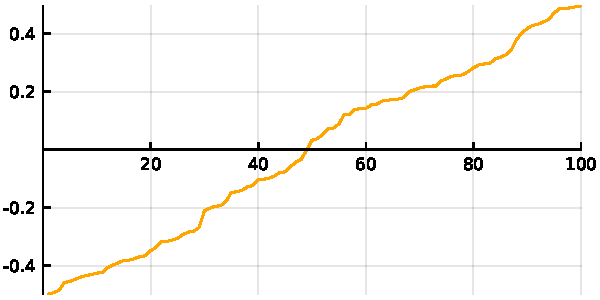
\includegraphics[width=\textwidth]{figures/density.pdf}

\end{frame}

\begin{frame}[fragile]{Maths}

The Input family of fonts has some support for Greek and mathematical
symbols:

\[
\frac{1}{N}\frac{\text{d}}{\text{d}t}N = N\left(r-\alert{\alpha N}\right)
\]

You can use \texttt{\textbackslash{}alert} within math blocks.

\end{frame}

\section{Using sections}\label{using-sections}

\begin{frame}[fragile]{Section titles}

Every section will have a small band with the background image.

They are first-level headers in markdown:

\begin{Shaded}
\begin{Highlighting}[]
\FunctionTok{# Section}

\FunctionTok{## Slide-title}

\NormalTok{Slide content}
\end{Highlighting}
\end{Shaded}

\end{frame}

\begin{frame}[fragile]{Code highlighting}

There is a customized color scheme for code highlighting.

\begin{Shaded}
\begin{Highlighting}[]
\NormalTok{α = }\FloatTok{2.0}
\NormalTok{b, c = }\StringTok{"abc"}\NormalTok{, }\CharTok{'c'}
\CommentTok{# This code does nothing (useful)}
\KeywordTok{for} \NormalTok{i }\KeywordTok{in} \FloatTok{1}\NormalTok{:}\FloatTok{10}
  \NormalTok{rand()}
  \NormalTok{@elapsed println(}\StringTok{"i:}\NormalTok{\textbackslash{}t}\StringTok{$i"}\NormalTok{)}
\KeywordTok{end}
\end{Highlighting}
\end{Shaded}

We can also use \alert{unicode characters}.

\end{frame}

\begin{frame}{Visual counter}

The circle next to the title of each slide moves forward at every slide
(including the section changes).

It is a useful visual key for how much slides are left.

\end{frame}

\begin{frame}{Output}

Pellentesque habitant morbi tristique senectus et netus et malesuada
fames ac turpis egestas. Morbi sollicitudin nisi vitae lorem interdum,
eget elementum quam elementum. Curabitur quis leo eu metus consequat
ultricies. Curabitur sit amet convallis risus. Cras vel arcu id risus
efficitur commodo et eget velit. Curabitur consequat eleifend magna, ut
ultricies lorem scelerisque eu. Mauris faucibus neque sit amet est
elementum, suscipit placerat est interdum. Phasellus sed convallis est.
Nunc fermentum convallis odio eget gravida. Duis venenatis dictum
tempor.

\end{frame}

\begin{frame}[fragile]{Background image}

The background image is generated from the \texttt{makebackground.jl}
file. It's the k-nearest neighbour graph of a series of random points.

The file is \texttt{background.png} -- it can be replaced by any file
\alert{as long
as} the replacement file is in the 16:10 format (for example, a 1600
\(\times\) 1000 image).

\end{frame}

\begin{frame}{Final slide}

The final slide displays the background picture.

This is to avoid the awkward ``Switching to black'' thing that happens
when there are no slides left.

\end{frame}

\section{Reproducible documents}\label{reproducible-documents}

\begin{frame}[fragile]{It's in the Makefile}

Documents \texttt{slides.Jmd} and \texttt{slides.Rmd} will be detected.

They will be converted to \texttt{slides.md} using either
\texttt{R}/\texttt{knitr} or \texttt{Julia}/\texttt{Weave.jl}.

\end{frame}

\section{Specific commands}\label{specific-commands}

\begin{frame}[fragile]{Cropped images}

\begincols
\column{0.68\textwidth}

The \texttt{roundpicture} command will display a picture, resized to fit
into a circle:

\begin{Shaded}
\begin{Highlighting}[]
\FunctionTok{\textbackslash{}roundpicture}\NormalTok{\{images/nb.png\}\{Optional text\}}
\end{Highlighting}
\end{Shaded}

Note that the image \alert{must} be a square.

\hfill\column{0.28\textwidth}

\roundpicture{images/nb.png}{}

\stopcols

\end{frame}

\begin{frame}[fragile]{Plain slide}

This will create a plain slide:

\begin{Shaded}
\begin{Highlighting}[]
\FunctionTok{## \{.plain\}}

\NormalTok{\textbackslash{}plain\{This is large text on the background image.\}}
\end{Highlighting}
\end{Shaded}

Note that the text within the \texttt{\textbackslash{}plain} command
\alert{must be \LaTeX}.

\end{frame}

\begin{frame}[plain]{}

\plain{This is large text on the background image.}

\end{frame}

\begin{frame}[plain]
  \begin{picture}(0,0)
    \put(-28.5,-175){%
      \pgfuseimage{titlebackground}
    }
  \end{picture}
\end{frame}

\end{document}
